\documentclass{beamer}
\usepackage{pdfpages}
%Imports and customization
\usepackage{tikz}
\usepackage{graphicx}
\usepackage{tikz-feynman}
\usepackage{ulem}
\usepackage{colortbl}
\graphicspath{ 
    {./images/}
}

\beamertemplatenavigationsymbolsempty
\setbeamertemplate{sidebar right}{}
\setbeamertemplate{footline}{
    \hfill\usebeamertemplate***{navigation symbols}
    \hspace{1cm}\insertframenumber{}/\inserttotalframenumber
}
\setbeamertemplate{caption}{\raggedright\insertcaption\par}
\setbeamersize{text margin left=4mm,text margin right=4mm} 

\setbeamerfont{itemize/enumerate body}{size=\scriptsize}
\setbeamerfont{itemize/enumerate subbody}{size=\scriptsize}
\setbeamerfont{itemize/enumerate subsubbody}{size=\scriptsize}


%Custom Macros
\newcommand{\statwarn}{
    \tiny \color{red} Absolute numbers here mean NOTHING. Plots are based on small (100k events) samples, and are highly biased. All that matters is relative position!
}


% WARNING: When using these commands, the image argument must
% NOT have spaces between itself and the braces
\newcommand{\fullscreenimage}[2]{
    \frame{
        \frametitle{#1} 
        \begin{figure}
        \includegraphics[height=0.9\textheight,width=\textwidth,keepaspectratio]{#2}
        \end{figure}
    }
}


\newcommand{\importpdf}[3]{
    \frame{
        \begin{columns}\column{\dimexpr\paperwidth-10pt}
        \begin{figure}
        \includegraphics[page=#2,height=0.8\textheight,width=\textwidth,keepaspectratio]{#1}
        \end{figure}

        {\tiny #3}
        \end{columns}
    }
}


\newcommand{\displayone}[3]{
    \frame{
        \frametitle{#1} 
        \begin{columns}
            \begin{column}{0.5\textwidth}
                #2
            \end{column}
            \begin{column}{0.5\textwidth}
                \begin{figure}
                    \includegraphics[width=\linewidth,height=\textheight,keepaspectratio]{#3}
                \end{figure}
            \end{column}
        \end{columns}
    }
}

\newcommand{\displayonelarge}[3]{
    \frame{
        \frametitle{#1} 
        \begin{columns}
            \begin{column}{0.3\textwidth}
                #2
            \end{column}
            \begin{column}{0.7\textwidth}
                \begin{figure}
                    \includegraphics[width=\linewidth,height=0.8\textheight,keepaspectratio]{#3}
                \end{figure}
            \end{column}
        \end{columns}
    }
}


\newcommand{\displaytwo}[4]{
    \frame{
        \frametitle{#1} 
        #2
        \begin{columns}
            \begin{column}{0.5\textwidth}
                \begin{figure}
                    \includegraphics[width=\linewidth,height=\textheight,keepaspectratio]{#3}
                \end{figure}
            \end{column}
            \begin{column}{0.5\textwidth}
                \begin{figure}
                    \includegraphics[width=\linewidth,height=\textheight,keepaspectratio]{#4}
                \end{figure}
            \end{column}
        \end{columns}
    }
}

\newcommand{\displaytwocaption}[6]{
    \frame{
        \frametitle{#1} 
        #2
        \begin{columns}
            \begin{column}{0.5\textwidth}
                \begin{figure}
                    \includegraphics[width=\linewidth,height=\textheight,keepaspectratio]{#3}
                    \caption{#4}
                \end{figure}
            \end{column}
            \begin{column}{0.5\textwidth}
                \begin{figure}
                    \includegraphics[width=\linewidth,height=\textheight,keepaspectratio]{#5}
                    \caption{#6}
                \end{figure}
            \end{column}
        \end{columns}
    }
}

\newcommand{\displaytwoVcaption}[6]{
    \frame{
        \begin{columns}
            \begin{column}{0.5\textwidth}
                \frametitle{#1} 
                #2
            \end{column}
            \begin{column}{0.5\textwidth}
                \begin{figure}
                    \includegraphics[width=\linewidth,height=0.3\textheight,keepaspectratio]{#3}
                    \caption{#4}
                \end{figure}

                \begin{figure}
                    \includegraphics[width=\linewidth,height=0.3\textheight,keepaspectratio]{#5}
                    \caption{#6}
                \end{figure}
            \end{column}
        \end{columns}
    }
}


\newcommand{\displaythree}[5]{
    \frame{
        \begin{columns}[T]
            \begin{column}{0.4\textwidth}
                {\usebeamercolor[fg]{title} \insertframetitle{#1} }\\
                \vspace{5mm}
                #2
            \end{column}
            \begin{column}{0.4\textwidth}
                \begin{figure}
                    \includegraphics[width=\linewidth,height=\textheight,keepaspectratio]{#3}
                \end{figure}
            \end{column}
        \end{columns}
        \begin{columns}[T]
            \begin{column}{0.4\textwidth}
                \begin{figure}
                    \includegraphics[width=\linewidth,height=\textheight,keepaspectratio]{#4}
                \end{figure}
            \end{column}
            \begin{column}{0.4\textwidth}
                \begin{figure}
                    \includegraphics[width=\linewidth,height=\textheight,keepaspectratio]{#5}
                \end{figure}
            \end{column}
        \end{columns}
    }
}


\newcommand{\displayfour}[5]{
    \frame{
        \frametitle{#1} 
        \begin{columns}[T]
            \begin{column}{0.4\textwidth}
                \begin{figure}
                    \includegraphics[width=\linewidth,height=\textheight,keepaspectratio]{#2}
                \end{figure}
            \end{column}
            \begin{column}{0.4\textwidth}
                \begin{figure}
                    \includegraphics[width=\linewidth,height=\textheight,keepaspectratio]{#3}
                \end{figure}
            \end{column}
        \end{columns}
        \begin{columns}[T]
            \begin{column}{0.4\textwidth}
                \begin{figure}
                    \includegraphics[width=\linewidth,height=\textheight,keepaspectratio]{#4}
                \end{figure}
            \end{column}
            \begin{column}{0.4\textwidth}
                \begin{figure}
                    \includegraphics[width=\linewidth,height=\textheight,keepaspectratio]{#5}
                \end{figure}
            \end{column}
        \end{columns}
    }
}


\newcommand{\pstrike}[2]{
    \only<-\the\numexpr#1-1>{#2}
    \only<#1->{\sout{#2}}
}


\newcommand{\announcesection}[1]{
    \section{#1}
    \frame{
        \begin{center}
            {\huge #1} 
        \end{center}
    }
}

\newcommand{\kvv}{\kappa_{2V}}
\newcommand{\kl}{\kappa_{\lambda}}
\newcommand{\kv}{\kappa_{V}}

\newcommand{\fkvv}[1]{\kappa_{2V,#1}}
\newcommand{\fkl} [1]{\kappa_{\lambda,#1}}
\newcommand{\fkv} [1]{\kappa_{V,#1}}

\newcommand{\importpdfwpages}[3]{
    \foreach \pageN in {#2,...,#3}{
        \importpdf{#1}{\pageN}{}
    }
}

\newcommand{\hyper}[2]{{\color{blue}\href{#1}{#2}}}



%Begin Presentation
\begin{document}
    \setbeamercolor{background canvas}{bg=}
    \title{1/2/3D VBF Combinations with the New May MC Production}
    \author{Chris Milke}
    \date{26 May, 2021}

    \frame{\titlepage}
    \frame{\frametitle{Overview} \tableofcontents}

    \section{Introduction}
    % Show the old math intro again
    \section{Linear Algebra}

% show diagrams with terms, then show squaring
\frame{
    \frametitle{3D Coupling Dependence}
    \begin{figure}
    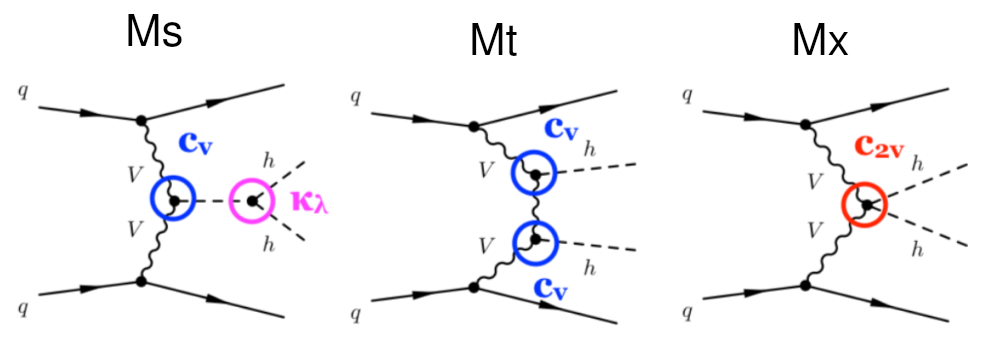
\includegraphics[width=0.6\linewidth,height=0.6\textheight,keepaspectratio]{vbf-hh_diagrams2b}
    \end{figure}
    $ \sigma = | \kv \kl M_s + \kv^2 M_t + \kvv M_x |^2 = $

    \vspace{10mm}

    $ \kv^2 \kl^2 M_s^2 + \kv^4 M_t^2 + \kvv^2 M_x^2 
    + \kv^3 \kl (M_s^* M_t + M_t^* M_s) 
    + \kv \kl \kvv (M_s^* M_x + M_x^* M_s ) 
    + \kv^2 \kvv (M_t^* M_x + M_x^* M_t )$

    \vspace{10mm}

    $ \sigma = \kv^2 \kl^2 a_1 + \kv^4 a_2 + \kvv^2 a_3 + \kv^3 \kl a_4 + \kv \kl \kvv a_5 + \kv^2 \kvv a_6 $
}

% convert to matrix, show nice matrix solution
\frame{
    \frametitle{Reweighting Solved via Linear Algebra}

    \begin{columns}[T]
        \begin{column}{0.18\textwidth}
            $ \vec{\sigma} = \begin{pmatrix} \sigma_1 \\
                \sigma_2 \\ \sigma_3 \\ \sigma_4 \\
                \sigma_5 \\ \sigma_6 \end{pmatrix} $
        \end{column}
        \begin{column}{0.15\textwidth}
            $ \vec{a} = \begin{pmatrix} a_1 \\ a_2 \\ a_3 \\ a_4 \\ a_5 \\ a_6 \end{pmatrix} $
        \end{column}
        \begin{column}{0.25\textwidth}
            $ \vec{f} = \begin{pmatrix} \kv^2 \kl^2 \\ \kv^4 \\ \kvv^2 \\ \kv^3 \kl \\ \kv \kl \kvv \\ \kv^2 \kvv \end{pmatrix} $
        \end{column}
        \begin{column}{0.4\textwidth}
            $ F = \begin{pmatrix}
                \vec{f}(\fkvv{1}, \fkl{1}, \fkv{1}) \\
                \vec{f}(\fkvv{2}, \fkl{2}, \fkv{2}) \\
                \vec{f}(\fkvv{3}, \fkl{3}, \fkv{3}) \\
                \vec{f}(\fkvv{4}, \fkl{4}, \fkv{4}) \\
                \vec{f}(\fkvv{5}, \fkl{5}, \fkv{5}) \\
                \vec{f}(\fkvv{6}, \fkl{6}, \fkv{6}) \\
            \end{pmatrix} $
        \end{column}
    \end{columns}

    \vspace{10mm}

    $ \vec{\sigma} = F \bullet \vec{a} \; \Longrightarrow \; \vec{a} = F^{-1} \bullet \vec{\sigma} $

    \vspace{10mm}

    $ \boxed{ \sigma(\kvv,\kl,\kv) = \vec{f}(\kvv,\kl,\kv) \bullet F^{-1} \bullet \vec{\sigma} } $
}


    % Show a quick look at the new sample combinatorics and the negative weight heatmap as reminder of how I pick things
    \frame{
    \frametitle{New MC Samples!}
    \begin{columns} \begin{column}{0.5\textwidth}
        \begin{center} 
            619 Possible Combinations of 6,\\
            250 Include SM Sample

            \resizebox{0.3\textheight}{!}{\begin{tabular}{ |l|l|l| }
                \hline
                \textbf {$\kappa_{2V}$} & \textbf {$\kappa_\lambda$} & \textbf {$\kappa_V$} \\
                \hline
                0    & 0   & 1   \\
                0    & 1   & 1   \\
                0.5  & 1   & 1   \\
                1    & 0   & 1   \\
                1    & 1   & 0.5 \\
                1    & 1   & 1   \\
                1    & 1   & 1.5 \\
                1    & 10  & 1   \\
                1    & 2   & 1   \\
                1.5  & 1   & 1   \\
                2    & 1   & 1   \\
                3    & 1   & 1   \\
                \hline
            \end{tabular}}
        \end{center}
    \end{column} \begin{column}{0.5\textwidth}
        {\footnotesize Rank combinations by the surface integral of the number of negative bins at each point at in the $\kappa$ parameter space (mutliplying by the $\kvv \times \kl$ ``area" of each square)}

        \begin{figure}
        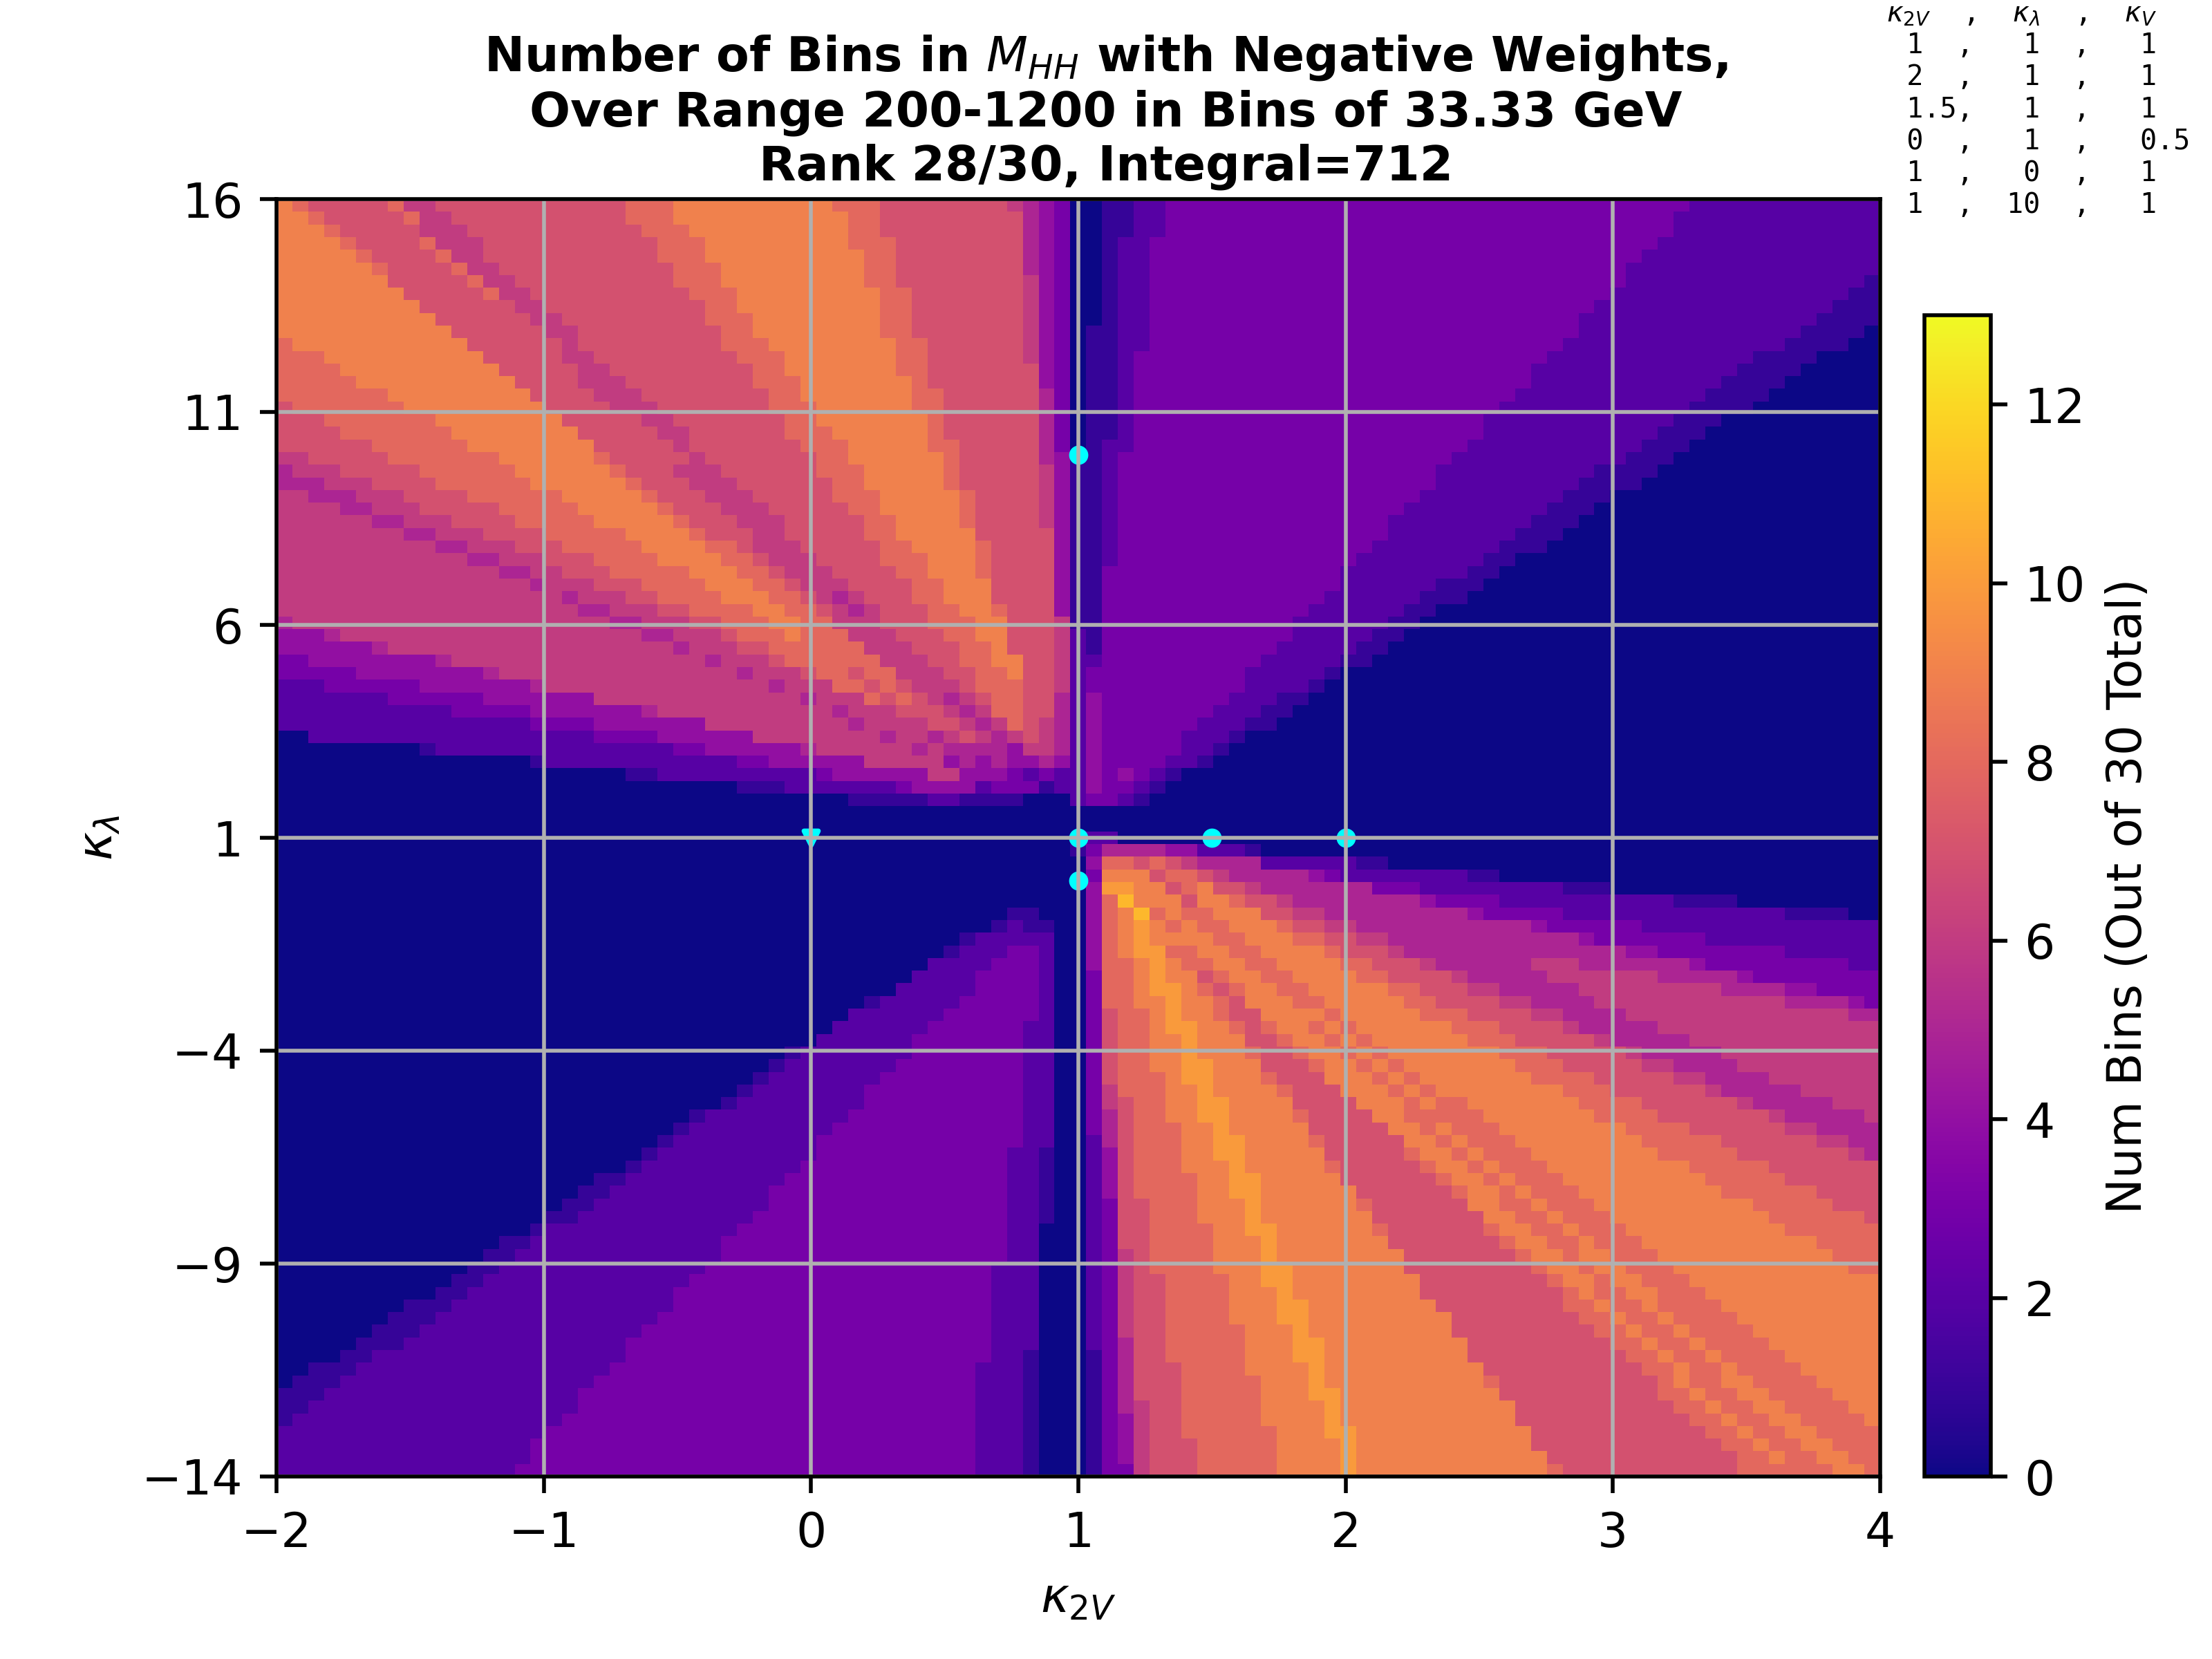
\includegraphics[width=\linewidth,height=\textheight,keepaspectratio]{negative_weights_rank027}
        \end{figure}
    \end{column} \end{columns}
}

\frame{
    \frametitle{Testing Specs}
    \begin{itemize} {
        \item All plots produced using non-min MC samples.
        \item Systematic samples caused problems, combinations (even in 1D) were terribly mismodelled everywhere
        \item I might just have read them wrong?
        \item Will check cryptotuples ASAP to ensure there are no similar issues with them
    } \end{itemize}


}



    % 1D klambda
    %   Show top three basis as bare dump
    %   Show mhh map of top two
    %   Show single validation of top two
    %   Show preview plots of top two
    \announcesection{$\kl$ 1D}

\frame{
    \frametitle{$\kl$ Bases}
    \begin{center} 

    3 Possible Bases
    \vspace{5mm}

    \begin{tabular}{ |l|l|l|l| }
        \hline
            \textbf {$\kl$ - 1} & \textbf {$\kl$ - 2} & \textbf {$\kl$ - 3} & \textbf {Nweight Int}\\
            \hline
            1   &  2  &  10  &    0.0 \\
            1   &  0  &  10  &    6.9 \\
            1   &  0  &  2   &   25.8 \\
            \hline
            \end{tabular}
    \end{center}
}

\frame{
    \frametitle{$\kl$ Top Two Bases}
    \begin{columns}
        \begin{column}{0.5\textwidth}
            \resizebox{\textwidth}{!}{ \begin{minipage}{1.0\textwidth}
            Rank 1 Basis Equation
            \vspace{10mm}

            {\tiny $\left(- \frac{\kappa_{\lambda}^{2}}{8} + \frac{11 \kappa_{\lambda}}{8} - \frac{5}{4}\right) \times \sigma{\left(1,2,1 \right)} +$

$ \left(\frac{\kappa_{\lambda}^{2}}{72} - \frac{\kappa_{\lambda}}{24} + \frac{1}{36}\right) \times \sigma{\left(1,10,1 \right)} +$

$ \left(\frac{\kappa_{\lambda}^{2}}{9} - \frac{4 \kappa_{\lambda}}{3} + \frac{20}{9}\right) \times \sigma{\left(1,1,1 \right)}$
}
            \end{minipage}}
        \end{column} \begin{column}{0.5\textwidth}
            \resizebox{\textwidth}{!}{ \begin{minipage}{1.0\textwidth}
            Rank 2 Basis Equation

            \vspace{10mm}

            {\tiny $\left(- \frac{\kappa_{\lambda}^{2}}{9} + \frac{10 \kappa_{\lambda}}{9}\right) \times \sigma{\left(1,1,1 \right)} +$

$ \left(\frac{\kappa_{\lambda}^{2}}{90} - \frac{\kappa_{\lambda}}{90}\right) \times \sigma{\left(1,10,1 \right)} +$

$ \left(\frac{\kappa_{\lambda}^{2}}{10} - \frac{11 \kappa_{\lambda}}{10} + 1\right) \times \sigma{\left(1,0,1 \right)}$
}
            \end{minipage}}
        \end{column}
    \end{columns}
}

\displaytwo{$m_{HH}$ Spectrum for Top 2 Bases}
{Red lines indicate basis samples, white patches indicate negative bins.}
{auto-kl_rank0}
{auto-kl_rank1}

\displayfour{$\kl$ Validation Plots}
{reco_mHH_compare_autokl01_cvv1p0cl0p0cv1p0}
{reco_mHH_compare_autokl01_cvv1p0cl10p0cv1p0}
{reco_mHH_compare_autokl01_cvv1p0cl1p0cv1p0}
{reco_mHH_compare_autokl01_cvv1p0cl2p0cv1p0}

\displayfour{$\kl$ Preview Plots}
{reco_mHH_compare_preview_autokl01_cvv1p0cl-14p0cv1p0}
{reco_mHH_compare_preview_autokl01_cvv1p0cl-11p0cv1p0}
{reco_mHH_compare_preview_autokl01_cvv1p0cl-8p0cv1p0}
{reco_mHH_compare_preview_autokl01_cvv1p0cl-5p0cv1p0}

\displayfour{$\kl$ More Preview Plots}
{reco_mHH_compare_preview_autokl01_cvv1p0cl-2p0cv1p0}
{reco_mHH_compare_preview_autokl01_cvv1p0cl4p0cv1p0}
{reco_mHH_compare_preview_autokl01_cvv1p0cl7p0cv1p0}
{reco_mHH_compare_preview_autokl01_cvv1p0cl13p0cv1p0}



    % 1D k2v
    %   Show top three basis as bare dump
    %   Show mhh map of top two
    %   Show all validation plots of top two
    %   Show preview plots of top two
    \announcesection{$\kvv$ 1D}

\frame{
    \frametitle{$\kvv$ Bases}
    \begin{center} 

    10 Possible Bases
    \vspace{5mm}

    \begin{tabular}{ |l|l|l|l| }
        \hline
            \textbf {$\kvv$ - 1} & \textbf {$\kvv$ - 2} & \textbf {$\kvv$ - 3} & \textbf {Nweight Int}\\
            \hline
                1  & 0.0  &  1.5  &  0.00 \\
                1  & 0.5  &  1.5  &  0.00 \\
                1  & 0.0  &  2.0  &  1.20 \\
                1  & 0.5  &  2.0  &  1.62 \\
                1  & 0.0  &  3.0  &  1.92 \\
                1  & 0.5  &  3.0  &  2.40 \\
                1  & 2.0  &  3.0  &  2.88 \\
                1  & 1.5  &  3.0  &  3.90 \\
                1  & 0.0  &  0.5  &  7.74 \\
                1  & 1.5  &  2.0  &  9.18 \\
            \hline
            \end{tabular}
    \end{center}
}

\frame{
    \frametitle{$\kvv$ Top Two Bases}
    \begin{columns}
        \begin{column}{0.5\textwidth}
            \resizebox{\textwidth}{!}{ \begin{minipage}{1.0\textwidth}
            Rank 1 Basis Equation
            \vspace{10mm}

            {\tiny $\left(- 2 \kappa_{2V}^{2} + 3 \kappa_{2V}\right) \times \sigma{\left(1,1,1 \right)} +$

$ \left(\frac{4 \kappa_{2V}^{2}}{3} - \frac{4 \kappa_{2V}}{3}\right) \times \sigma{\left(\frac{3}{2},1,1 \right)} +$

$ \left(\frac{2 \kappa_{2V}^{2}}{3} - \frac{5 \kappa_{2V}}{3} + 1\right) \times \sigma{\left(0,1,1 \right)}$
}
            \end{minipage}}
        \end{column} \begin{column}{0.5\textwidth}
            \resizebox{\textwidth}{!}{ \begin{minipage}{1.0\textwidth}
            Rank 2 Basis Equation

            \vspace{10mm}

            {\tiny $\left(- \frac{4 \kappa_{2V}^{2}}{3} + \frac{16 \kappa_{2V}}{3} - 4\right) \times \sigma{\left(\frac{3}{2},1,1 \right)} +$

$ \left(\frac{\kappa_{2V}^{2}}{3} - \frac{5 \kappa_{2V}}{6} + \frac{1}{2}\right) \times \sigma{\left(3,1,1 \right)} +$

$ \left(\kappa_{2V}^{2} - \frac{9 \kappa_{2V}}{2} + \frac{9}{2}\right) \times \sigma{\left(1,1,1 \right)}$
}
            \end{minipage}}
        \end{column}
    \end{columns}
}

\displaytwo{$m_{HH}$ Spectrum for Top 2 Bases}
{Red lines indicate basis samples, white patches indicate negative bins (there are none for these bases).}
{auto-k2v_rank0}
{auto-k2v_rank1}

\displaythree{$\kvv$ Validation Plots}{}
{reco_mHH_compare_autok2v01_cvv0p0cl1p0cv1p0}
{reco_mHH_compare_autok2v01_cvv0p5cl1p0cv1p0}
{reco_mHH_compare_autok2v01_cvv1p0cl1p0cv1p0}

\displaythree{$\kvv$ More Validation Plots}{}
{reco_mHH_compare_autok2v01_cvv1p5cl1p0cv1p0}
{reco_mHH_compare_autok2v01_cvv2p0cl1p0cv1p0}
{reco_mHH_compare_autok2v01_cvv3p0cl1p0cv1p0}

\displayfour{$\kvv$ Preview Plots}
{reco_mHH_compare_preview_autok2v01_cvv-2p0cl1p0cv1p0}
{reco_mHH_compare_preview_autok2v01_cvv-1p4cl1p0cv1p0}
{reco_mHH_compare_preview_autok2v01_cvv-0p8cl1p0cv1p0}
{reco_mHH_compare_preview_autok2v01_cvv0p4cl1p0cv1p0}

\displayfour{$\kvv$ More Preview Plots}
{reco_mHH_compare_preview_autok2v01_cvv1p6cl1p0cv1p0}
{reco_mHH_compare_preview_autok2v01_cvv2p2cl1p0cv1p0}
{reco_mHH_compare_preview_autok2v01_cvv2p8cl1p0cv1p0}
{reco_mHH_compare_preview_autok2v01_cvv3p4cl1p0cv1p0}



    % 1D k2v multibasis
    %   Show plot of bases, equations, and range
    %   Show mhh map of this and 1D
    %   Show preview plots
    \announcesection{$\kvv$ 1D Multi-Basis}

\frame{
    \frametitle{$\kvv$ Multi-Basis}
    \begin{center} 

    Historically used for $\kvv$ scan. Uses 3 different bases in different ranges.
    \vspace{5mm}

    \begin{tabular}{ |l|l|l|l| }
        \hline
            \textbf {$\kvv$ - 1} & \textbf {$\kvv$ - 2} & \textbf {$\kvv$ - 3} & \textbf {Range}\\
            \hline
                    1  &  0.5  &  0    &  $     \kvv \leq 0 $ \\
                    2  &  1.5  &  1    &  $ 0 < \kvv \leq 2 $ \\
                    3  &  2    &  1.5  &  $ 2 < \kvv $ \\
            \hline
            \end{tabular}
    \end{center}
}

\displaytwo{$m_{HH}$ Spectrum for Multi-Basis VS Single Basis}
{Red lines indicate basis samples, white patches indicate negative bins.}
{projectionscan_k2v_multicompare}
{c2v_9S_projection}


\displayfour{$\kvv$ Multi-Basis Vs Single Basis Preview Plots}
{preview_reco_mHH_multibasis_cvv-2p00cl1p00cv1p00}
{preview_reco_mHH_multibasis_cvv-1p40cl1p00cv1p00}
{preview_reco_mHH_multibasis_cvv-0p80cl1p00cv1p00}
{preview_reco_mHH_multibasis_cvv-0p20cl1p00cv1p00}

\displaythree{$\kvv$ More Multi-Basis Vs Single Basis Preview Plots}{}
{preview_reco_mHH_multibasis_cvv0p40cl1p00cv1p00}
{preview_reco_mHH_multibasis_cvv1p60cl1p00cv1p00}
{preview_reco_mHH_multibasis_cvv2p20cl1p00cv1p00}

\displaythree{$\kvv$ Even More Multi-Basis Vs Single Basis Preview Plots}{}
{preview_reco_mHH_multibasis_cvv2p80cl1p00cv1p00}
{preview_reco_mHH_multibasis_cvv3p40cl1p00cv1p00}
{preview_reco_mHH_multibasis_cvv4p00cl1p00cv1p00}


    % 3D
    %   Show full equation and Nweight integrals for top two
    %   Show Nweight heat maps of top two
    %   Show all validation plots of top two
    %   Show preview plots of top two
    %   Show 
    \announcesection{$\kvv, \kl, \kv$ 3D Full Scan}

\frame{
    \frametitle{6-Term Bases}

    Over 600 Valid Combinations, 250 of which contain the SM sample.
    \vspace{5mm}

    Top 10 Bases. Samples displayed as $(\kvv, \kl, \kv)$
    \vspace{3mm}

    \resizebox{0.8\textwidth}{!}{ \begin{minipage}{1.0\textwidth}
    \begin{tabular}{ |l|l|l|l|l|l|c| }
        \hline
            \textbf {Sample 1} & \textbf {Sample 2} & \textbf {Sample 3} &
            \textbf {Sample 4} & \textbf {Sample 5} & \textbf {Sample 6} &
            \textbf {Nweight Int}\\
            \hline
            (1, 1, 1) & (0.5, 1, 1) & (3, 1, 1) & (1, 2, 1 ) & (1, 10, 1) & (0, 0, 1) &  323 \\
            (1, 1, 1) & (0.5, 1, 1) & (3, 1, 1) & (1, 0, 1 ) & (1, 10, 1) & (0, 0, 1) &  343 \\
            (1, 1, 1) & (0.5, 1, 1) & (1.5, 1, 1) & (1, 2, 1 ) & (1, 10, 1) & (0, 0, 1) &  362 \\
            (1, 1, 1) & (0.5, 1, 1) & (2, 1, 1) & (1, 2, 1 ) & (1, 10, 1) & (0, 0, 1) &  365 \\
            (1, 1, 1) & (0.5, 1, 1) & (1.5, 1, 1) & (1, 0, 1 ) & (1, 10, 1) & (0, 0, 1) &  387 \\
            (1, 1, 1) & (0, 1, 1) & (1, 2, 1) & (1, 10, 1) & (1, 1, 0.5)  & (0, 0, 1) &  390 \\
            (1, 1, 1) & (0.5, 1, 1) & (2, 1, 1) & (1, 0, 1 ) & (1, 10, 1) & (0, 0, 1) &  394 \\
            (1, 1, 1) & (0.5, 1, 1) & (1, 2, 1) & (1, 10, 1) & (1, 1, 0.5)  & (0, 0, 1) &  397 \\
            (1, 1, 1) & (0.5, 1, 1) & (1, 0, 1) & (1, 10, 1) & (1, 1, 0.5)  & (0, 0, 1) &  398 \\
            (1, 1, 1) & (0, 1, 1) & (3, 1, 1) & (1, 2, 1 ) & (1, 10, 1) & (0, 0, 1) &  400 \\
            \hline
    \end{tabular}
    \end{minipage}}
}

\frame{ \frametitle{6-Term Top Two Bases}
    Rank 1\\
    \vspace{3mm}
    \resizebox{0.8\textwidth}{!}{ \begin{minipage}{1.0\textwidth}
    {\tiny $\left(2 \kappa_{2V}^{2} - 2 \kappa_{2V} \kappa_{V}^{2} - 3 \kappa_{2V} \kappa_{V} \kappa_{\lambda} + 3 \kappa_{V}^{3} \kappa_{\lambda}\right) \times \sigma{\left(\frac{1}{2},1,1 \right)} +$

$ \left(2 \kappa_{2V}^{2} - 2 \kappa_{2V} \kappa_{V}^{2} - \kappa_{2V} \kappa_{V} \kappa_{\lambda} + \kappa_{V}^{3} \kappa_{\lambda}\right) \times \sigma{\left(\frac{3}{2},1,1 \right)} +$

$ \left(- \frac{5 \kappa_{2V} \kappa_{V}^{2}}{4} + \frac{5 \kappa_{2V} \kappa_{V} \kappa_{\lambda}}{4} + \frac{\kappa_{V}^{3} \kappa_{\lambda}}{8} - \frac{\kappa_{V}^{2} \kappa_{\lambda}^{2}}{8}\right) \times \sigma{\left(1,2,1 \right)} +$

$ \left(- \kappa_{2V} \kappa_{V}^{2} + \kappa_{2V} \kappa_{V} \kappa_{\lambda} + \kappa_{V}^{4} - \kappa_{V}^{3} \kappa_{\lambda}\right) \times \sigma{\left(0,0,1 \right)} +$

$ \left(\frac{\kappa_{2V} \kappa_{V}^{2}}{36} - \frac{\kappa_{2V} \kappa_{V} \kappa_{\lambda}}{36} - \frac{\kappa_{V}^{3} \kappa_{\lambda}}{72} + \frac{\kappa_{V}^{2} \kappa_{\lambda}^{2}}{72}\right) \times \sigma{\left(1,10,1 \right)} +$

$ \left(- 4 \kappa_{2V}^{2} + \frac{56 \kappa_{2V} \kappa_{V}^{2}}{9} + \frac{16 \kappa_{2V} \kappa_{V} \kappa_{\lambda}}{9} - \frac{28 \kappa_{V}^{3} \kappa_{\lambda}}{9} + \frac{\kappa_{V}^{2} \kappa_{\lambda}^{2}}{9}\right) \times \sigma{\left(1,1,1 \right)}$
}
    \end{minipage}}

    \vspace{7mm}

    Rank 2\\
    \vspace{3mm}
    \resizebox{0.8\textwidth}{!}{ \begin{minipage}{1.0\textwidth}
    {\tiny $\left(\frac{2 \kappa_{2V}^{2}}{3} - \frac{2 \kappa_{2V} \kappa_{V}^{2}}{3} - \frac{\kappa_{2V} \kappa_{V} \kappa_{\lambda}}{3} + \frac{\kappa_{V}^{3} \kappa_{\lambda}}{3}\right) \times \sigma{\left(2,1,1 \right)} +$

$ \left(\frac{4 \kappa_{2V}^{2}}{3} - \frac{4 \kappa_{2V} \kappa_{V}^{2}}{3} - \frac{8 \kappa_{2V} \kappa_{V} \kappa_{\lambda}}{3} + \frac{8 \kappa_{V}^{3} \kappa_{\lambda}}{3}\right) \times \sigma{\left(\frac{1}{2},1,1 \right)} +$

$ \left(- \frac{5 \kappa_{2V} \kappa_{V}^{2}}{4} + \frac{5 \kappa_{2V} \kappa_{V} \kappa_{\lambda}}{4} + \frac{\kappa_{V}^{3} \kappa_{\lambda}}{8} - \frac{\kappa_{V}^{2} \kappa_{\lambda}^{2}}{8}\right) \times \sigma{\left(1,2,1 \right)} +$

$ \left(- \kappa_{2V} \kappa_{V}^{2} + \kappa_{2V} \kappa_{V} \kappa_{\lambda} + \kappa_{V}^{4} - \kappa_{V}^{3} \kappa_{\lambda}\right) \times \sigma{\left(0,0,1 \right)} +$

$ \left(\frac{\kappa_{2V} \kappa_{V}^{2}}{36} - \frac{\kappa_{2V} \kappa_{V} \kappa_{\lambda}}{36} - \frac{\kappa_{V}^{3} \kappa_{\lambda}}{72} + \frac{\kappa_{V}^{2} \kappa_{\lambda}^{2}}{72}\right) \times \sigma{\left(1,10,1 \right)} +$

$ \left(- 2 \kappa_{2V}^{2} + \frac{38 \kappa_{2V} \kappa_{V}^{2}}{9} + \frac{7 \kappa_{2V} \kappa_{V} \kappa_{\lambda}}{9} - \frac{19 \kappa_{V}^{3} \kappa_{\lambda}}{9} + \frac{\kappa_{V}^{2} \kappa_{\lambda}^{2}}{9}\right) \times \sigma{\left(1,1,1 \right)}$
}
    \end{minipage}}
}

\displaythree{6-Term Negative Weight Heatmap}
{ \tiny
    New production (below) performs signficantly \textit{worse} than old production (right).
    \vspace{3mm}

    I think this is to do with the absence of the $\kvv,\kl,\kv = [0, 1, 0.5]$ sample, but this is unclear.
}
{old_negative_weights_toprank000}
{negative_weights_toprank0}
{negative_weights_toprank1}

\displayfour{6-Term Validation Plots}
{reco_mHH_compare_auto_top_3D_0-1_cvv0p0cl0p0cv1p0}
{reco_mHH_compare_auto_top_3D_0-1_cvv0p0cl1p0cv1p0}
{reco_mHH_compare_auto_top_3D_0-1_cvv0p5cl1p0cv1p0}
{reco_mHH_compare_auto_top_3D_0-1_cvv1p0cl0p0cv1p0}

\displayfour{6-Term More Validation Plots}
{reco_mHH_compare_auto_top_3D_0-1_cvv1p0cl10p0cv1p0}
{reco_mHH_compare_auto_top_3D_0-1_cvv1p0cl1p0cv0p5}
{reco_mHH_compare_auto_top_3D_0-1_cvv1p0cl1p0cv1p0}
{reco_mHH_compare_auto_top_3D_0-1_cvv1p0cl1p0cv1p5}

\displayfour{6-Term Even More Validation Plots}
{reco_mHH_compare_auto_top_3D_0-1_cvv1p0cl2p0cv1p0}
{reco_mHH_compare_auto_top_3D_0-1_cvv1p5cl1p0cv1p0}
{reco_mHH_compare_auto_top_3D_0-1_cvv2p0cl1p0cv1p0}
{reco_mHH_compare_auto_top_3D_0-1_cvv3p0cl1p0cv1p0}



\displayfour{6-Term Preview Plots (1/4)}
{reco_mHH_compare_preview_auto_top_3D_0-1_cvv-1p5cl-3p0cv1p0}
{reco_mHH_compare_preview_auto_top_3D_0-1_cvv-1p5cl-9p0cv1p0}
{reco_mHH_compare_preview_auto_top_3D_0-1_cvv-1p5cl14p0cv1p0}
{reco_mHH_compare_preview_auto_top_3D_0-1_cvv-1p5cl5p0cv1p0}

\displayfour{6-Term Preview Plots (2/4)}
{reco_mHH_compare_preview_auto_top_3D_0-1_cvv0p5cl-3p0cv1p0}
{reco_mHH_compare_preview_auto_top_3D_0-1_cvv0p5cl-9p0cv1p0}
{reco_mHH_compare_preview_auto_top_3D_0-1_cvv0p5cl14p0cv1p0}
{reco_mHH_compare_preview_auto_top_3D_0-1_cvv0p5cl5p0cv1p0}

\displayfour{6-Term Preview Plots (3/4)}
{reco_mHH_compare_preview_auto_top_3D_0-1_cvv2p0cl-3p0cv1p0}
{reco_mHH_compare_preview_auto_top_3D_0-1_cvv2p0cl-9p0cv1p0}
{reco_mHH_compare_preview_auto_top_3D_0-1_cvv2p0cl14p0cv1p0}
{reco_mHH_compare_preview_auto_top_3D_0-1_cvv2p0cl5p0cv1p0}

\displayfour{6-Term Preview Plots (4/4)}
{reco_mHH_compare_preview_auto_top_3D_0-1_cvv3p5cl-3p0cv1p0}
{reco_mHH_compare_preview_auto_top_3D_0-1_cvv3p5cl-9p0cv1p0}
{reco_mHH_compare_preview_auto_top_3D_0-1_cvv3p5cl14p0cv1p0}
{reco_mHH_compare_preview_auto_top_3D_0-1_cvv3p5cl5p0cv1p0}

    \displayfour{3D Combination VS 1D Combination}
{reco_mHH_1-2D_compare_cvv0p0cl1p0cv1p0}
{reco_mHH_1-2D_compare_cvv1p0cl0p0cv1p0}
{reco_mHH_1-2D_compare_cvv2p0cl1p0cv1p0}
{reco_mHH_1-2D_compare_cvv3p0cl1p0cv1p0}


\frame{
    \frametitle{3D Equation VS 1D Equations}
    \begin{columns}
        \begin{column}{0.7\textwidth}
            \resizebox{0.8\textwidth}{!}{ \begin{minipage}{1.0\textwidth}
            { \footnotesize 
                The optimal 6-Term basis uses all the samples present in the two individual 1D combinations.

                When combining samples along an axis, all the coefficients associated with that coupling drop to zero.

                \vspace{2mm}
                e.g. for the $\sigma{\left(\frac{1}{2},1,1 \right)}$ coefficient for $\kvv=\kv=1$:
                \vspace{3mm}

                $\left(2 \kappa_{2V}^{2} - 2 \kappa_{2V} \kappa_{V}^{2} - 3 \kappa_{2V} \kappa_{V} \kappa_{\lambda} + 3 \kappa_{V}^{3} \kappa_{\lambda}\right)$

                $ = \left(2 \cdot 1^{2} - 2 \cdot 1 \cdot 1^{2} - 3 \cdot 1 \cdot 1 \cdot \kappa_{\lambda} + 3 \cdot 1^{3} \cdot \kappa_{\lambda}\right) $

                $ = \left(2 - 2 - 3 \kappa_{\lambda} + 3 \kappa_{\lambda}\right) = 0$
            \vspace{3mm}

            Thus, along the $\kl$ and $\kvv$ axes, the optimal 6-term equation is mathematically identical to the optimal 1D equations.
            }
            \vspace{7mm}

            Rank 1 6-Term Equation
            \vspace{5mm}

            {\tiny $\left(2 \kappa_{2V}^{2} - 2 \kappa_{2V} \kappa_{V}^{2} - 3 \kappa_{2V} \kappa_{V} \kappa_{\lambda} + 3 \kappa_{V}^{3} \kappa_{\lambda}\right) \times \sigma{\left(\frac{1}{2},1,1 \right)} +$

$ \left(2 \kappa_{2V}^{2} - 2 \kappa_{2V} \kappa_{V}^{2} - \kappa_{2V} \kappa_{V} \kappa_{\lambda} + \kappa_{V}^{3} \kappa_{\lambda}\right) \times \sigma{\left(\frac{3}{2},1,1 \right)} +$

$ \left(- \frac{5 \kappa_{2V} \kappa_{V}^{2}}{4} + \frac{5 \kappa_{2V} \kappa_{V} \kappa_{\lambda}}{4} + \frac{\kappa_{V}^{3} \kappa_{\lambda}}{8} - \frac{\kappa_{V}^{2} \kappa_{\lambda}^{2}}{8}\right) \times \sigma{\left(1,2,1 \right)} +$

$ \left(- \kappa_{2V} \kappa_{V}^{2} + \kappa_{2V} \kappa_{V} \kappa_{\lambda} + \kappa_{V}^{4} - \kappa_{V}^{3} \kappa_{\lambda}\right) \times \sigma{\left(0,0,1 \right)} +$

$ \left(\frac{\kappa_{2V} \kappa_{V}^{2}}{36} - \frac{\kappa_{2V} \kappa_{V} \kappa_{\lambda}}{36} - \frac{\kappa_{V}^{3} \kappa_{\lambda}}{72} + \frac{\kappa_{V}^{2} \kappa_{\lambda}^{2}}{72}\right) \times \sigma{\left(1,10,1 \right)} +$

$ \left(- 4 \kappa_{2V}^{2} + \frac{56 \kappa_{2V} \kappa_{V}^{2}}{9} + \frac{16 \kappa_{2V} \kappa_{V} \kappa_{\lambda}}{9} - \frac{28 \kappa_{V}^{3} \kappa_{\lambda}}{9} + \frac{\kappa_{V}^{2} \kappa_{\lambda}^{2}}{9}\right) \times \sigma{\left(1,1,1 \right)}$
}
            \end{minipage}}
        \end{column} \begin{column}{0.4\textwidth}
            \resizebox{0.8\textwidth}{!}{ \begin{minipage}{1.0\textwidth}
            Rank 2 $\kvv$ 1-D Equation

            \vspace{5mm}

            {\tiny $\left(- \frac{4 \kappa_{2V}^{2}}{3} + \frac{16 \kappa_{2V}}{3} - 4\right) \times \sigma{\left(\frac{3}{2},1,1 \right)} +$

$ \left(\frac{\kappa_{2V}^{2}}{3} - \frac{5 \kappa_{2V}}{6} + \frac{1}{2}\right) \times \sigma{\left(3,1,1 \right)} +$

$ \left(\kappa_{2V}^{2} - \frac{9 \kappa_{2V}}{2} + \frac{9}{2}\right) \times \sigma{\left(1,1,1 \right)}$
}
            \end{minipage}}
            \vspace{10mm}

            \resizebox{0.8\textwidth}{!}{ \begin{minipage}{1.0\textwidth}
            Rank 1 $\kl$ 1-D Equation

            \vspace{5mm}

            {\tiny $\left(- \frac{\kappa_{\lambda}^{2}}{8} + \frac{11 \kappa_{\lambda}}{8} - \frac{5}{4}\right) \times \sigma{\left(1,2,1 \right)} +$

$ \left(\frac{\kappa_{\lambda}^{2}}{72} - \frac{\kappa_{\lambda}}{24} + \frac{1}{36}\right) \times \sigma{\left(1,10,1 \right)} +$

$ \left(\frac{\kappa_{\lambda}^{2}}{9} - \frac{4 \kappa_{\lambda}}{3} + \frac{20}{9}\right) \times \sigma{\left(1,1,1 \right)}$
}
            \end{minipage}}
        \end{column}
    \end{columns}
}




    %Conclusion 
    \section{Conclusion}
    \frame{
        \frametitle{Conclusion}
        \begin{itemize} {
            \item New Samples are in, with many bases to choose from
            \item 1D $\kvv$ and $\kl$ bases look good
            \item Multi-basis combination looks questionable, maybe just use single basis
            \item 2D basis is worse than before unfortunately, may need to get creative
        } \end{itemize}
    }

    %\announcesection{Backup}

\end{document}
